\documentclass[conference]{IEEEtran}

\usepackage{adjustbox}
\usepackage{amsmath}
\usepackage{caption}
\usepackage[nocompress]{cite}
\usepackage{geometry}
\usepackage{graphicx}
\usepackage{pdflscape}
\usepackage{pgfgantt}
\usepackage{ragged2e}
\usepackage{url}
\usepackage{verbatim}

\begin{comment}

# Submission (26th Sept): pdf - Tabula
	<30MB
	Bundle code as ZIP in electronic submission

>18000, 20000 words

# Assessment Criteria
* Technical content
    * Well read and knowledgeable in the project's subject area
    * Good insight into the project's specific topic
    * Effective analysis of the problems and issues relating to the project's aims
    * Quality of design work and appropriate choice of methods and tools
    * Effective testing/validation regime
    * Quality of results and analysis
    * Critical evaluation of the project
    * Quality of practical/technical work and overall level of technical achievement.
* Project management and organization
    * Good consistent progress
    * Initially unforeseen problems well detected and overcome
    * Necessary research, analysis and design work completed
    * Completeness of project overall.
* Communication skills
    * Clear exposition of the aims, achievements and limitations of the project
    * Coherence, structure and composition of report
    * Software and hardware appropriate documented
    * Readability and appropriate length.

\end{comment}

\begin{comment}
    * Abstract
    * Introduction
        * Background
        * Related Work
    * Project Management
        * Gantt Chart
        * Git repo
        * Latex
    * Investigation
        * gprof
    * Design
    * Implementation
    * Testing
    * Conclusion
        * Limitations
        * Improvements
        * Future Work
    * References
\end{comment}


\begin{document}
\newgeometry{vmargin=2.25cm, hmargin=2.25cm}
\title{Integrating CUDA into SNAP}


\author{\IEEEauthorblockN{Andrew Lamzed-Short}
\IEEEauthorblockA{ID: 1897268}}


\maketitle

%%%%%%%%%%%%%%%%%%%%%%%%%%%%%%%%%%%%%%%%%%

\begin{abstract}

Mini-applications (``miniapps'') are small-scale, representative versions of large-scale pieces of scientific or engineering-focused software that seek to model the performance of an algorithm or program without actually executing the larger program. This project seeks to examine the effects of altering the codebase of one such miniapp called ``SNAP'' from utilising only traditional processing cores to incorporating a mixture of traditional computation in addition to offloading applicable workloads to graphical processing cores, aiming to leverage their increased throughput and capabilities for single instruction, multiple data (SIMD) assignments. Ultimately the hope is to examine the performance of the resulting program to ascertain whether the modification is beneficial to the runtime of the algorithm, justifying if this change can be reflected in the larger-scale software SNAP represents.

To this end, this dissertation details a brief description to the field of High-Performance Computing (``HPC''), along with an introduction and description of the new field of miniapps. Overall aims of the project are outlined before related work in the field of miniapps, application modelling, and related HPC disciplines and projects is presented The target miniapp SNAP is discussed in addition to outlining the objectives of what the project aims to achieve by modifying it. Current efforts and progress are detailed and reflected upon against the timeline offered in the project proposal previously submitted as part of this project/module. Finally, further work and a future timeline is described.

\end{abstract}

%%%%%%%%%%%%%%%%%%%%%%%%%%%%%%%%%%%%%%%%%%

\section{Introduction}\label{introduction}

\subsection{Background}

Modern, frontier-level science calls for large-scale, ambitious projects to answer some of the toughest questions. These projects often involve vast, complex simulations of natural phenomena, from modelling a human brain in one-to-one detail to answer questions about how memory works and how consciousness arises, to modelling the oceans to understand and make predictions about weather and climate change.

One of the predominant questions when designing these simulations is what architecture is best to run this program/suite of programs on. Different workloads and algorithms are designed for and benefit from certain types of computer architecture – some algorithms lend themselves well to being distributed over many cores, whereas others do not. Supercomputers of significant power are leveraged today for the foremost problems of our time: weather simulation and prediction\cite{metoffice}, human brain simulation\cite{humanbrain}, and simulated nuclear weapons testing\cite{nuclear}. The current state-of-the-art supercomputers, their power consumption and performance, are published in a list known as the ``Top500”\cite{top500}, with the most powerful supercomputer to date being ``Summit” housed at Oak Ridge National Laboratory, which can reach a performance of 143,500 Tflops/s\footnote{A ``flop” is an abbreviation for 1 floating-point, numerical operation, and a Tflop is a Teraflop, or $10\textsuperscript{12}$ floating point operations.} utilising 2,397,824 processing cores.

% [Supercomputer Architecture]
In general, supercomputers are comprised of numerous server racks housing many full computer systems – each one containing several CPUs, several graphics card, memory, and high-speed networking capabilities – all interconnected via a high-speed network to allow for communication and cooperation. The topology of the network connecting the computers can vary but two types tend to prevail: computer clusters, and grid computing. Clusters are composed of numerous components that are connected via a centralised resource management system to act as one individual system, with multiple clusters connected by a high-speed local area network (e.g. all in a single site) for low-latency communication; grid computing utilises clusters that are distributed geographically with the underlying assumption that a user of the system need not worry about where the computing resources they are going to be utilising are located – this provides reliability and access to and provision of additional resources on demand. The advantage of cluster computing for supercomputing over grid-based computing systems is stability and very low latency between nodes, as there isn’t a need for a high-speed internet connection between sites (also allowing the system to be air-gapped from the outside world for security purposes).

% [OpenMP and MPI – Software and programming paradigms to take advantage of this]
Since the era of Moore’s Law with respect to single-threaded/core workloads is coming to an end\cite{mooreslaw}, processors nowadays tend to have multiple cores, with consumer-grade electronics averaging four cores per chip, as can be seen in Figure \ref{fig:cpu_diagram} which details the architecture of a quad-core Intel Core i7 CPU. In addition to hyper-threading (2 threads per physical core), CPUs can have an effective/``logical” core count of twice that. Programming workloads to take advantage of this hardware-based parallelism can be challenging, and parallelising code over multiple nodes in a supercomputer can be even more so. This is where libraries such as OpenMP\footnote{\url{https://www.openmp.org/}} and MPI\footnote{\url{https://www.mpi-forum.org/}} come in. These are Application Programming Interfaces (APIs) that define how such a complex parallelisation system is to work, and each has multiple open-source implementations that allow for programmers to convert their code from single-threaded to multi-threaded over multiple clusters. It is these technologies predominantly that a large proportion of HPC applications are built with.

% \footnote{\url{https://m.hexus.net/tech/reviews/cpu/16187-intel-core-i7-x58-chipset-systems-go-fsb-invited}}
\begin{figure}
\centering
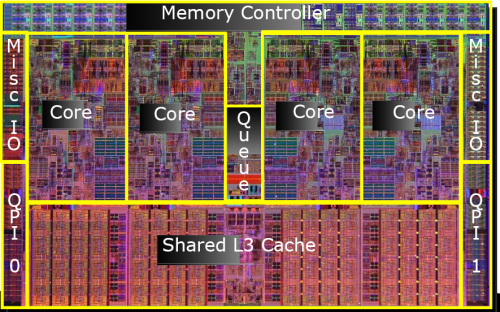
\includegraphics[width=0.45\textwidth]{images/cpu_diagram.png}
\caption{Quad-core Intel Core i7 CPU Architecture Diagram}
\label{fig:cpu_diagram}
\end{figure}

% [Use of GPUs – GPU Architecture]
Graphical Processing Units (GPU) are a newer technology than CPUs and serve a dedicated purpose of taking instructions from the CPU and performing multiple, hardware-based mathematical operations for translating three-dimensional shapes and coordinates into two-dimensional projections for rendering to a display, and runs multiple small programs called ``shaders” to handle colour and lighting. Due to the sheer amount of mathematical calculations that need to be performed to display something onto a display, GPUs are architected differently to a CPU. Modern graphics cards, such as NVIDIA’s Turing architecture, pictured in Figure \ref{fig:gpu_diagram}, are composed of multiple stream processors, each divided into hundreds of small cores which perform a single integer or floating-point operation. This stream processing approach allows for vast parallel computation over a large dataset in a paradigm called ``single instruction multiple data” (SIMD).

This parallelism was previously reserved for image and video processing but a few years ago NVIDIA released their CUDA API\cite{cuda_talk}\cite{CUDA} which allows developers to leverage the stream processing nature of the GPU for general-purpose computation. Scientific workloads from biomedical imaging\cite{luebke2008cuda} to deep learning\cite{tang2013deep} are now done on the GPU, and modern supercomputers, such as Summit, are built with large numbers of GPUs to accelerate workloads and perform previously-impossible simulations and workloads.

% \footnote{\url{https://devblogs.nvidia.com/nvidia-turing-architecture-in-depth/}}
\begin{figure}
\centering
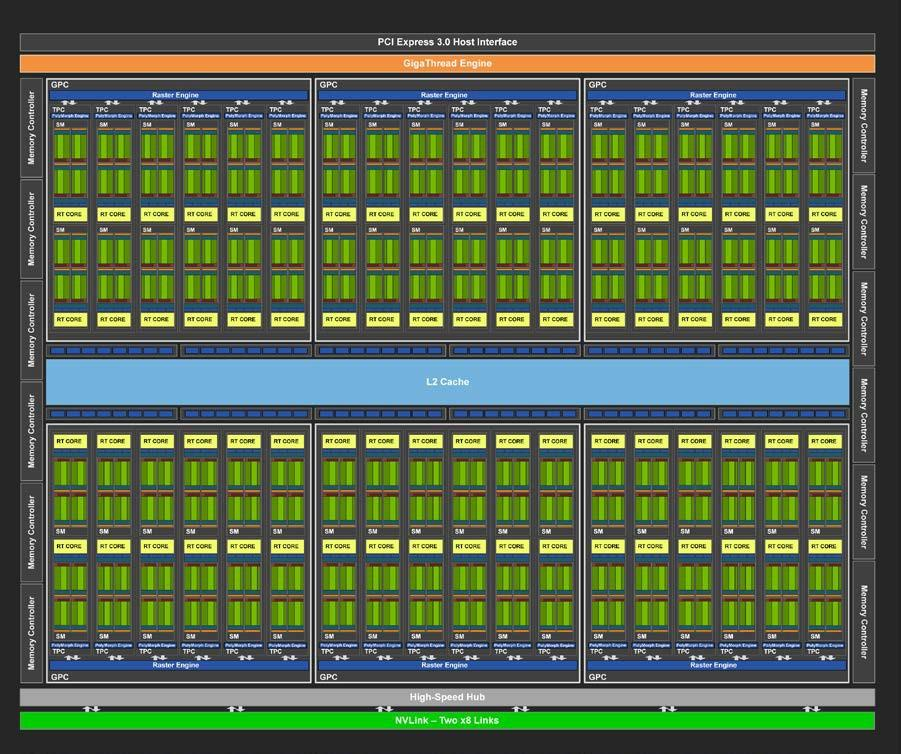
\includegraphics[width=0.45\textwidth]{images/gpu_diagram.jpg}
\caption{NVIDIA Turing GPU Streaming Multiprocessor Architecture Diagram}
\label{fig:gpu_diagram}
\end{figure}

% Miniapps
Mini-applications (``miniapp”) are a new area within the field of High Performance Computing (HPC). These applications are small, self-contained proxies for real applications (typically relating to simulation of physical phenomena) to quickly and concisely explore a parameter space, leading to focused and interesting performance results to investigate potential scaling and run-time issues or trade-offs\cite{miniapps}. Miniapps capture the behaviour and essence of their parent applications primarily because of two characteristics of many applications running on distributed systems: the performance of an application will mainly be constituted by the performance of a small subset of the code, and many of the physical models that constitute the rest of the application are mathematically distinct and generally have similar performance characteristics\cite{miniapps}.

\subsection{Objectives}

The SN (Discrete Ordinates) Application Proxy (SNAP) is a miniapp that acts as a proxy for discrete ordinates particle transport. It is modelled off another production simulation program developed by the Los Alamos National Laboratory (``LANL'') called PARTISN, which solves the linear Boltzmann transport equation (TE)\footnote{Boltzmann Equation: \url{https://en.wikipedia.org/wiki/Boltzmann_equation}\raggedright}, simulating neutron criticality and time-independent neutron leakage problems\cite{partisn} in a multi-dimensional phase space. SNAP is a proxy to PARTISN because it provides a concise solution to a discretised, approximated version (though with no real-world relevance) of the same problem PARTISN solves, providing the same data layout, the same number of operations, and loads elements into arrays in approximately the same order.

The SNAP algorithm works by defining the phase space as seven dimensions: three in space (x, y, z), two in angle (octants, angles), one in energy (groups, or energy-based bins of particles), and one of time (time step). SNAP sweeps across the spatial mesh, starting in each of the octants proceeding towards the antipodal octant, performing a time-dependent calculation in each cell using information from the previous time-step and surrounding cells. This motion forms a wave-front motion that sweeps across the three-dimensional space from corner to corner, with work being divided along each diagonal for parallel execution

With this miniapp in mind, we define three key objectives that the project shall solve. Taken together, these will provide a holistic overview as to the validity and efficacy of this approach of converting CPU-bound parallelised algorithms to utilise the GPU instead (where appropriate). With the SNAP algorithm and open-source repository (specifically the C-based port of the code) in mind, the three objectives are:

\begin{itemize}

\item To instrument, profile, and analyse the current implementation of the code in order to identify areas of the code in which it would be applicable and beneficial to convert to CUDA-based parallelisation.

\item Using the identified areas found in problem 1, to fork the current C-based port of the SNAP GitHub repository\footnote{\url{https://github.com/lanl/SNAP}} and convert the candidate components and routines from OpenMP to utilise the CUDA libraries instead.

\item Following the reimplementation of the algorithm to CUDA technology, the last step is to analyse and evaluate the efficiency and efficacy of the new solution in comparison to the previous CPU-based approach. Ideally, a theoretical maximum efficiency of the approach will also be calculated mathematically, and the actual implementation compared against this as another measure of success.

\end{itemize}

%%%%%%%%%%%%%%%%%%%%%%%%%%%%%%%%%%%%%%%%%%

\subsection{Related Work}

A seminal work in the field of miniapps was written by Heroux et al\cite{miniapps}, defining the paradigm. Their Mantevo miniapp suite has show successful development of miniapps, such as MiniFE for finite element analysis and MiniMD for molecular dynamics simulations, to demonstrate their versatility and applicability. Others have demonstrated such success in other areas, such as Mallinson et al with ``CloverLeaf”\cite{mallinson2013cloverleaf}, and Los Alamos National Lab (\url{https://www.lanl.gov/projects/codesign/proxy-apps/lanl/index.php}). Miniapps have been shown to produce similar performance characteristics to their fully-fledged counterparts\cite{miniapps}, adding to the efficacy of the paradigm.

General-purpose simulations on GPUs have been studied for a long time, with GPUs being a core part of modern computing clusters\cite{debardeleben2013gpu}. Strong-scaling across multiple GPUs\cite{glaser2015strong} is the ideal approach. Consideration is taken also for conversion of existing codebases\cite{zhou2011gpu} and new, bespoke solutions designed with GPU architecture utilisation in mind\cite{glaser2015strong}. Bespoke solutions offer superior code architecture and speed, meaning calculation of theoretical maximum performance increase for a pre-existing code base will have to take this into account.

Writing GPU targeted miniapps in a developing area of work. Baker et al\cite{baker2012high} discuss implementation details of converting the KBA sweep algorithm of the Denovo code system to run on NVIDIA’s Titan GPU. Mallison et al\cite{mallinson2013cloverleaf} demonstrate too with CloverLeaf the performance advantages GPU-based architecture targeting can have over purely CPU-based versions. It is important to note that these performance increases might not necessarily be completely reflected in SNAP’s algorithm due to other considerations, such as the scaling characteristics of the algorithm\cite{shoukourian2014predicting} and communication technologies as highlighted by Glaser et al\cite{glaser2015strong}.

Performance of miniapps with respect to CPU- and GPU-based parallelisation frameworks have been explored previously and show promising results which add credence to the motivation of this project. Notably Martineau et al\cite{martineau2017productivity} reached the conclusion that compiling miniapps to CUDA resulted in greater efficiencies compared to other targets, though care is needed to consider the implementation (especially with respect to data accesses) to avoid the compiler introducing performance penalties.

Development of the solution must still mimic the behaviour of the original application however, so care must be taken to preserve this. Heroux et al\cite{miniapps} and Messer et al\cite{messer2015developing} outline the fundamental principles that a miniapp must adhere to and the considerations of forming a miniapp from the base application – all of which would help form testing criteria for this project and future projects to help preserve results and intrinsic behaviour.

%%%%%%%%%%%%%%%%%%%%%%%%%%%%%%%%%%%%%%%%%%

\section{Project Management}\label{projectmgmt}

Several factors need to be considered when developing a software project. Management of time constraints is discussed first as producing a novel software project as part of an entire Masters course will run into difficulty - mostly with conflicting or overlapping deadlines but also due to the inevitable problems associated with any software development project. Following on from this, it is also key to highlight how the code was managed and versioned so as to preserve the history of changes and the progression of the project, should ideas need to be experimented with or code recovered should anything unforeseen occur.

\subsection{Time Constraints}

Time constraints are always a pressing and important factor to consider when starting a large project. The external largest constraints imposed on this project would be the time required to complete several overlapping courseworks for various MSc modules, in addition to setting aside time to adequately prepare for and take the end of year exams in June and July. To manage these obstacles, the timeline presented in Figure \ref{fig:gantt_chart} was developed early on in the research phase of the project to delineate when and how long certain key stages of development were to last for, with built-in highlighting of potential speed-bumps to this project's progression.

\begin{figure*}[h!]
    % \begin{adjustbox}{max width=0.7\textwidth}
        \centering
        \ganttset{calendar week text=\small{\startday}}
        \begin{ganttchart}[
            hgrid,x unit=0.1cm,
            hgrid style/.style={draw=black!5, line width=.75pt},
            vgrid={draw=none,draw=none},
            bar label node/.style={text width=2cm,align=right,font=\scriptsize\RaggedLeft,anchor=east},
            group label node/.style={text width=2cm,align=right,font=\bf\scriptsize\RaggedLeft,anchor=east},
            time slot format=little-endian]{01-05-2019}{26-09-2019}
        \gantttitlecalendar{month=shortname, week=4} \\
        \ganttgroup{Total Duration}{01-07-2019}{12-09-19}\\
        % Investigation and Design
        \ganttgroup{Investigation and Design}{01-07-19}{31-07-19}\\
        \ganttbar{Collating Stacktraces and Data}{01-07-19}{20-07-19}\\
        \ganttbar{Mathematical Model}{01-07-19}{27-07-19}\\
        \ganttbar{Finalise CUDA Education}{01-07-19}{31-07-19}\\
        % Design and implementation
        \ganttgroup{Design and Implementation}{01-07-19}{30-08-19}\\
        % Testing
        \ganttgroup{Testing}{15-07-19}{14-08-19}\\
        \ganttbar{Local Profiling and Benchmarking}{15-07-19}{14-08-19}\\
        \ganttbar{Cluster Profiling and Benchmarking}{14-07-19}{14-08-19}\\
        % Dissertation
        \ganttgroup{Dissertation}{26-08-19}{12-09-19}\\
        \ganttbar{Writing}{26-08-19}{10-09-19}\\
        \ganttbar{Proof Reading and Editing}{5-09-19}{12-09-19}
        \end{ganttchart}
    % \end{adjustbox}
    
    \caption{The Proposed Timeline of this Project}
    \label{fig:gantt_chart}
\end{figure*}

\subsection{Source Control}

Github



\subsection{Hardware and Software Setup}

\subsubsection{Visual Studio Code}
\begin{itemize}
    \item Cross-platform
    \item Automatable
    \item Extensions
\end{itemize}

\subsubsection{Hardware}

For local testing

\begin{itemize}
    \item Intel® Core™ i7-6700K CPU, clock speed of 4GHz. It is a quad-core CPU with hyperthreading enabled for an apparent core count of 8.
    \item NVIDIA GeForce GTX 1070 graphics card. Pascal architecture that supports the CUDA Compute functionality, 1.5Ghz base core clock, 8GB of GDDR5 memory, and 15 streaming multi-processors.
    \item 16GB of DDR4 RAM
    \end{itemize}


%%%%%%%%%%%%%%%%%%%%%%%%%%%%%%%%%%%%%%%%%%

\section{Investigation}\label{investigation}

\subsection{SNAP Repository Cloning and Documentation Review}

Initial plans involved gaining a fundamental understanding of the nature of the algorithms and data structures that the SNAP program utilises in order to effectively emulate and model its larger counterpart program. LANL provide the full FORTRAN90 source code, in addition to several ports into other, different languages, in the GitHub repository located at \url{https://www.github.com/lanl/snap/}. For the purposes of this project, it will be Intel's C-based port that shall be modified and examined due to ease of use for compilation and finding the appropriate tooling (compilers, syntax highlighters etc.) as well as increased familiarity with the language over FORTRAN90.

The entire repository was forked on GitHub for the purposes of modification. It can be found at \url{https://www.github.com/alshort/snap}. All non-C-based ports were removed from the repository in addition to any miscellaneous files and documentation as these were superfluous. Only the \texttt{qasnap/} and the \texttt{src/} directories (of Intel's code) were kept as these would be the only necessary sets of code needed to build, execute, and test SNAP and this project's proposed modifications.

In the main repository, various presentations and documentation are provided that discuss the reasoning behind creating SNAP, background behind PARTISN and the code SNAP was seeking to model, as well as an overview of some of the implementation details of the main constituent of the approach LANL and Intel took: the ``sweep'' algorithm.

\subsection{Execution, Profiling, and Investigation of Code}

\subsubsection{Compilation}

Intel chose to target the C-based port of SNAP towards Intel-based CPUs, hence the decision, as outlined in section \ref{projectmgmt}, to use a machine to locally test the program with having an Intel Core i7-6700K. This decision was made due to the original port writers' knowledge of the benefits that the architecture and proprietary improvements could bring to a strictly MPI-based implementation of SNAP.

GNU make is used to compile all facets of the program, with the main compiler being \texttt{mpiicc}. Whilst \texttt{gcc} is typically used to compile regular, standard C and C++ code, \texttt{icc} is Intel's C++ compiler that was built in order to specifically optimise code to run on Intel-created architectures. This includes optimisations for how memory is specifically accessed, how thread-based parallelisation is handled with regards to the OpenMP specification, data layout improvements, and support for modern iterations of C++ language specifications\footnote{\url{https://software.intel.com/en-us/c-compilers}}. \texttt{mpiicc} is an HPC-specific message-passing library built for use with the \texttt{icc} program (in particular its C-based capabilities). This library implements the Message Passing Interface (MPI) specification version 3.1\cite{intel-mpi-ref} to allow for bi-directional inter-process communication, regardless of how those processes are mapped to the underlying hardware.

Whilst provided in an operation state, this provision is predicated on the correct resources and dependencies being installed and linked up on the executing system. Installation of Intel's MPI libraries is straight-forward but ensuring that they will operate correctly when called is an issue. This

\subsubsection{Execution}

% different threads, input data, averaging

\subsection{gprof}

% Print out of "example" analysis

\subsection{Learning CUDA}

% ...
% "CUDA by Example" book

%%%%%%%%%%%%%%%%%%%%%%%%%%%%%%%%%%%%%%%%%%

\section{Design}

\begin{itemize}
    \item Mathematical model of ideal circumstances
    \item Code analysis
    \item 
\end{itemize}

\subsection{Mathematical Model}

% ...

\subsection{Test Harness}




%%%%%%%%%%%%%%%%%%%%%%%%%%%%%%%%%%%%%%%%%%


\section{Implementation}

\begin{itemize}
    \item Intel C MPI library
    \item Externalised CUDA algorithms
    \item nvcc and mpiicc
\end{itemize}

%%%%%%%%%%%%%%%%%%%%%%%%%%%%%%%%%%%%%%%%%%

\section{Testing}

\begin{itemize}
    \item Test Plan
    \item Local Testing
\end{itemize}


%%%%%%%%%%%%%%%%%%%%%%%%%%%%%%%%%%%%%%%%%%

\section{Conclusion}

\subsection{Limitations}

\subsection{Improvements}

\subsection{Further Work}

%%%%%%%%%%%%%%%%%%%%%%%%%%%%%%%%%%%%%%%%%%

\bibliographystyle{ieeetr}
\bibliography{dissertation}

\end{document}